\subsubsection{Wyszukiwanie Obiektów}
Podczas programowania w Unity, efektywne wyszukiwanie obiektów w scenie jest kluczowe dla wydajności gry. Unikamy zasobożernych funkcji, takich jak \textbf{FindObjectOfType}, szczególnie w każdej klatce, aby uniknąć zbędnego obciążenia. Ostatecznie wyeliminowaliśmy wszystkie użycia tej funkcji z kilku prostych powodów, ale m.in. dlatego, że funkcja ta przeszukuje całą scenę (mówimy tu o wszystkich obiektach gry i o wszystkich ich komponentach!) oraz nie jest ograniczona do konkretnego obszaru lub hierarchii.\\ \\
Zamiast tego, zalecamy korzystanie z bardziej efektywnych metod, takich jak:
\begin{itemize}
    \item \textbf{Bezpośrednie Referencje w Edytorze Unity:} Przypisywanie referencji bezpośrednio w inspektorze Unity może być bardzo efektywne. Jeśli dany obiekt jest dostępny bezpośrednio poprzez referencję, nie trzeba korzystać z funkcji wyszukujących.
    \item \textbf{GetChild:} Funkcja pozwalająca na odnalezienie konkretnego dziecka obiektu, co jest przydatne, gdy hierarchia obiektów jest złożona.
    \item \textbf{GetComponent:} Pozwala na bezpośrednie odnalezienie komponentu przypisanego do obiektu. Jest to efektywna metoda, zwłaszcza gdy wiemy, że dany obiekt posiada określony komponent.
    \item \textbf{GetComponentInParent:} Metoda umożliwiająca znalezienie komponentu w hierarchii rodzica obiektu.
    \item \textbf{GetComponentInChildren:} Funkcja wyszukująca komponenty wśród dzieci danego obiektu.
    \item \textbf{FindGameObjectWithTag:} Efektywne wyszukiwanie obiektów po tagu. Jest to skuteczna metoda, jeśli obiekty są odpowiednio oznaczone tagami.
    \item \textbf{Find:} Możemy używać ogólnego wyszukiwania obiektów, takiego jak Find, w celu znalezienia obiektu po jego nazwie. Należy jednak używać go z umiarem, aby uniknąć nadmiernego obciążenia.
\end{itemize}
Optymalnym rozwiązaniem jest również projektowanie systemu, w którym unikamy częstego wyszukiwania obiektów w czasie rzeczywistym. Zamiast tego, stosujmy strategie takie jak cachowanie referencji, używanie menedżerów lub struktur organizacyjnych w scenie, aby minimalizować liczbę operacji wyszukiwania. To podejście przyczyni się do płynności działania gry, zwłaszcza w przypadku dużych projektów.
\begin{figure}[h]
    \centering
    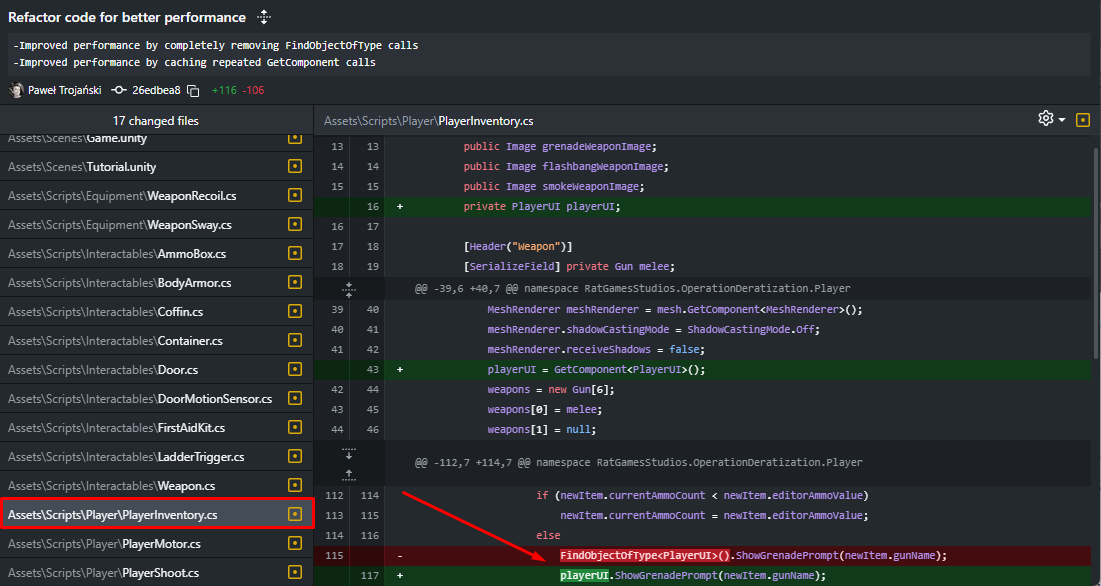
\includegraphics[width=1\linewidth]{Images/findObjectsOptimization.png}
    \caption{Optymalizacja pozyskiwania obiektów - porzucenie wywołań FindObjectOfType}
\end{figure}
\FloatBarrier

\subsubsection{Konstruktor Łańcucha Znaków}
\textbf{String Builder} to klasa w języku C\#, która umożliwia dynamiczne tworzenie, manipulowanie i modyfikowanie łańcuchów znaków. Główną różnicą między String Builder a standardowymi łańcuchami znaków (typ string) jest to, że String Builder jest mutowalny, co oznacza, że można go modyfikować bez tworzenia nowych instancji obiektów za każdym razem, gdy dokonywane są zmiany. \\ \\
\begin{enumerate}
    \item \textbf{Zalety String Buildera}
        \begin{itemize}
        \item \textbf{Efektywność pamięciowa:} W przypadku operacji na łańcuchach znaków, szczególnie gdy wymagane są powtarzane modyfikacje, String Builder oferuje znaczną efektywność pamięciową. Ponieważ obiekty typu string są niemodyfikowalne, każda operacja modyfikacji tworzy nowy obiekt. String Builder minimalizuje ten problem, pozwalając na modyfikację istniejącego obiektu bez konieczności tworzenia nowego za każdym razem.
        \item \textbf{Szybkość operacji modyfikacji:} Operacje modyfikacji, takie jak dodawanie, usuwanie lub zamiana znaków, są szybsze w przypadku String Builder niż dla typu string. W przypadku typu string, każda operacja modyfikacji tworzy nowy obiekt, co wpływa na wydajność, szczególnie w przypadku dużej liczby operacji.
        \item \textbf{Efektywność czasowa:} Dla operacji, które wymagają wielokrotnych modyfikacji, String Builder jest bardziej efektywny czasowo niż konkatenacja łańcuchów znaków (string + string). Konkatenacja za każdym razem tworzy nowy obiekt, co może prowadzić do kosztownych operacji kopiowania danych.
        \end{itemize}
    \item \textbf{Zastosowanie String Buildera}
        \begin{itemize}
        \item \textbf{Budowanie długich łańcuchów znaków:} Jeśli musisz dynamicznie budować długi łańcuch znaków, String Builder jest bardziej efektywny niż konkatenacja standardowych łańcuchów.
        \item \textbf{Częste modyfikacje tekstu:} W przypadku, gdy tekst podlega częstym zmianom, a konieczność tworzenia nowych obiektów jest nieefektywna, String Builder pozwala na płynne modyfikacje bez nadmiernego obciążenia pamięciowego.
        \item \textbf{Wydajne składanie wiadomości lub komunikatów:} W przypadku tworzenia komunikatów, logów lub innych dynamicznych komunikatów tekstowych, String Builder umożliwia efektywne tworzenie i modyfikowanie treści.
        \end{itemize}
    \item \textbf{Tworzenie Obiektu String Buildera}
        String Builder może być inicjowany różnymi sposobami. Poniżej przedstawiono jedną z metod tworzenia obiektu String Builder:
        \begin{verbatim}
            StringBuilder stringBuilder = new StringBuilder();
        \end{verbatim}
        Ten konstruktor tworzy pusty obiekt String Builder, który może być następnie modyfikowany przez różne operacje, takie jak dodawanie, usuwanie czy zamiana znaków.
        \begin{figure}[h]
            \centering
            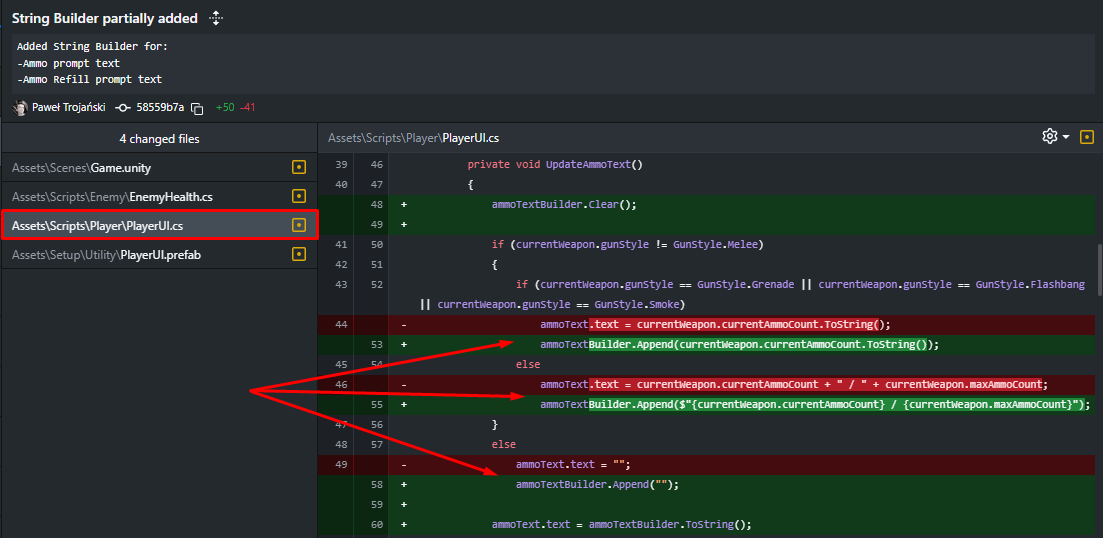
\includegraphics[width=1\linewidth]{Images/stringBuilder.png}
            \caption{Optymalizacja modyfikowania ciągów znaków - zastosowanie String Buildera}
        \end{figure}
\end{enumerate}
\FloatBarrier

\subsubsection{Pola Statyczne Obiektów}
Pola statyczne mogą być używane w celu przechowywania danych, które są wspólne dla wszystkich instancji danej klasy. Omówimy, kiedy i jak używać pól statycznych w celu zoptymalizowania zarządzania danymi w grze.
\begin{figure}[h]
    \centering
    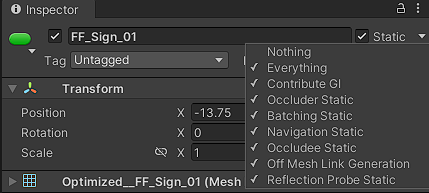
\includegraphics{Images/staticField.png}
    \caption{Odpowiednie wykorzystanie pola Static na obiekcie}
\end{figure}
\paragraph{Opcje Statycznych Pól Obiektów w Unity}\hspace{-1em} -- Statyczne pola obiektów w Unity oferują kilka opcji do kontrolowania zachowania obiektu w scenie. Oto opcje i ich znaczenia:
\begin{itemize}
    \item \textbf{Nothing:} Obiekt nie przyczynia się do statycznego zbiorczego renderowania (batching), eliminowania elementów niewidocznych (occlusion culling) ani globalnego oświetlenia (GI).
    \item \textbf{Everything:} Obiekt uczestniczy w batchingu, occlusion cullingu oraz GI.
    \item \textbf{Contribute GI:} Obiekt przyczynia się do obliczeń GI, ale nie uczestniczy w batchingu ani occlusion cullingu.
    \item \textbf{Occluder Static:} Obiekt działa jako zakrywacz dla statycznych obliczeń occlusion culling.
    \item \textbf{Batching Static:} Obiekt uczestniczy w batchingu, ale nie w GI ani occlusion cullingu.
    \item \textbf{Navigation Static:} Obiekt jest uwzględniany w generowaniu statycznej siatki nawigacyjnej.
    \item \textbf{Occludee Static:} Obiekt jest brany pod uwagę w occlusion cullingu, ale nie działa jako zakrywacz.
    \item \textbf{Off Mesh Link Generation:} Obiekt jest uwzględniany w generowaniu połączeń międzymeshowych dla nawigacji.
    \item \textbf{Reflection Probe Static:} Obiekt przyczynia się do statycznych obliczeń sond odbicia.
\end{itemize}

\subsubsection{Pola GPU Instancing}
Aktywowanie opcji GPU Instancing dla powtarzających się obiektów umożliwia renderowanie ich jednym wywołaniem, co przyśpiesza proces renderowania. Poniżej przedstawiamy konfigurację materiału w celu zastosowania tej techniki.
\begin{figure}[h]
    \centering
    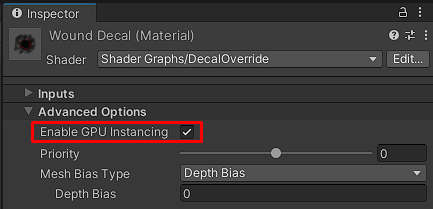
\includegraphics[width=0.85\linewidth]{Images/gpuInstanceOptimization.png}
    \caption{Renderowanie obiektów z użyciem GPU Instancing}
\end{figure}

\subsubsection{Wypiekanie Świateł} \label{subsubsec:bakingLights}
Wypiekanie świateł to proces wstępnych obliczeń oświetlenia, co może znacznie poprawić wydajność renderowania w czasie rzeczywistym. Przedstawimy korzyści i kroki do przeprowadzenia wypiekania świateł w projekcie.
\begin{itemize}
    \item \textbf{Poprawiona Wydajność Renderowania w Czasie Rzeczywistym:} Poprzez wstępne obliczenia informacji oświetleniowej, zmniejsza się konieczność obliczeń w czasie rzeczywistym podczas rozgrywki, co przekłada się na płynniejszą wydajność renderowania.
    \item \textbf{Spójność Oświetlenia:} Wypiekanie świateł zapewnia spójność oświetlenia pomiędzy scenami, poprawiając jednolity wygląd i utrzymując bardziej wyszukany charakter wizualny.
    \item \textbf{Zwiększone Detale i Cienie: } Wypiekanie oświetlenia pozwala uzyskać skomplikowane detale i realistyczne cienie, przyczyniając się do bardziej immersyjnego i atrakcyjnego otoczenia.
    \item \textbf{Optymalizacja dla Urządzeń Nisko-Wydajnych:} Wypiekanie świateł może być szczególnie korzystne dla optymalizacji projektów skierowanych na urządzenia nisko-wydajne, zapewniając lepsze doświadczenie użytkownika na różnych rodzajach sprzętu.
    \item \textbf{Przewidywalne Wyniki Oświetleniowe:} Ponieważ oświetlenie jest wstępnie obliczane, można osiągnąć przewidywalne i możliwe do odtworzenia wyniki oświetleniowe, co ułatwia precyzyjne dostrojenie wizualnej estetyki projektu.
\end{itemize}
Dzięki wykorzystaniu wypiekania świateł można znaleźć równowagę między jakością wizualną a wydajnością renderowania, tworząc bardziej przyjemne doświadczenie dla graczy.
\begin{figure}[h]
    \centering
    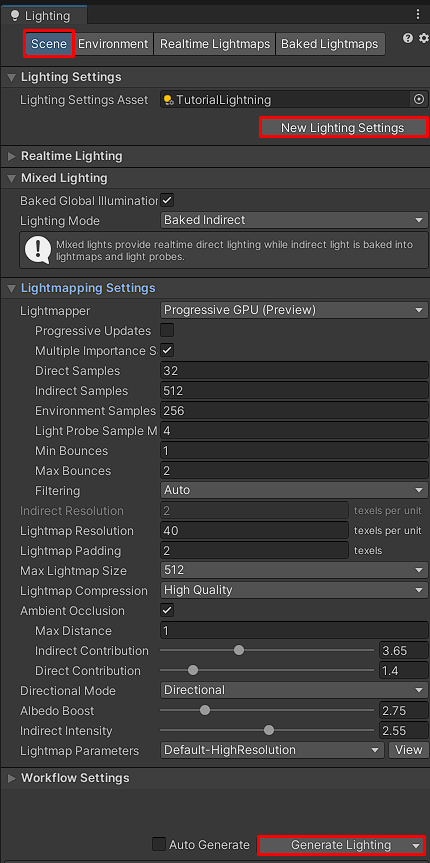
\includegraphics[height=1\linewidth]{Images/lightningWindow.png}
    \caption{Zakładka Scene ustawień oświetlenia, w której tworzymy plik dla sceny, a następnie konfigurujemy parametry i na koniec klikamy w Generate Lighting}
\end{figure}
\begin{figure}[h]
    \centering
    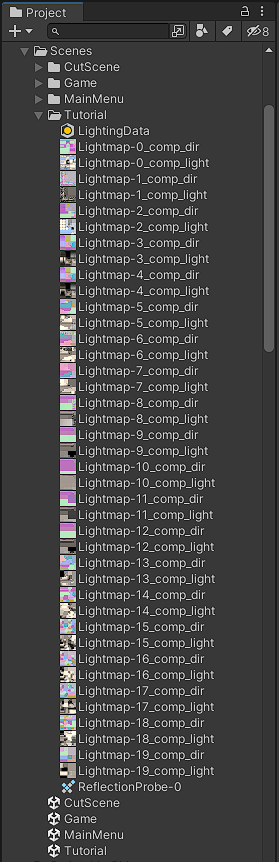
\includegraphics[height=0.95\linewidth]{Images/lightningSettingsFolder.png}
    \caption{Katalog zawierający wszystkie pliki wypieczonego oświetlenia}
\end{figure}
\begin{figure}[h]
    \centering
    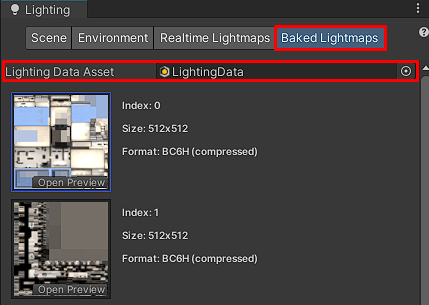
\includegraphics[width=0.5\linewidth]{Images/bakedLightmaps.png}
    \caption{Zakładka Baked Lightmaps okna oświetlenia, w której sprawdzimy wszystkie wygenerowane dane oświetlenia dla wybranego pliku oświetlenia sceny}
\end{figure}
\FloatBarrier
\begin{figure}[h]
    \centering
    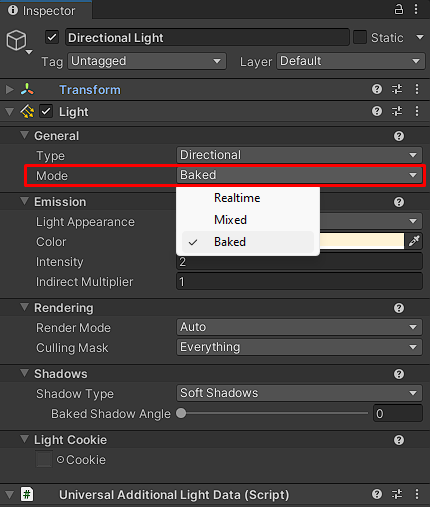
\includegraphics[scale=0.4]{Images/lightSettingsInspector.png}
    \caption{Konfiguracja obiektów światła - ustawiamy tryb Mixed lub Bake by móc korzystać z wypieczonych map}
\end{figure}
\begin{figure}[h]
    \centering
    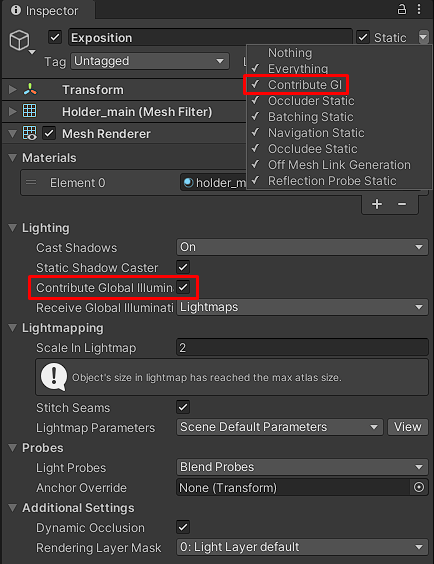
\includegraphics[scale=0.4]{Images/contributeGI.png}
    \caption{Ustawienia statycznego obiektu, który ma brać udział w wypiekaniu światła}
\end{figure}

% \subsubsection{Wypiekanie Okluzji}
% Eliminowanie elementów niewidocznych (occlusion culling) pozwala na pominięcie renderowania obiektów niewidocznych z perspektywy kamery. Przedstawimy zastosowanie tej techniki do optymalizacji renderowania.
% To-Do In-Game as well

\subsubsection{Optymalizacja Meshów}
Wprowadzenie odpowiednich optymalizacji meshów może znacznie poprawić wydajność renderowania. Poniżej przedstawiamy przykładowy obiekt, który wykorzystuje opcjonalnie zoptymalizowany mesh i Mesh Collider z low poly wersją oryginału. Mesh Collider dodatkowo może być skonfigurowany poprzez zaznaczenie pola "Convex". Zaleca się używanie tej opcji w przypadku, gdy mesh jest całkowicie zamknięty, bez otworów czy dziur. Dodatkowo używamy ze skryptu OptimizeMesh.cs z paczki dostępnej na Asset Store: \href{https://assetstore.unity.com/packages/tools/modeling/mesh-optimizer-154517}{\texttt{Mesh Optimizer}}. Ten skrypt umożliwia dynamiczną optymalizację mesha przy użyciu suwaka "Quality". Zmniejszając wartość suwaka, można skutecznie obniżyć jakość mesha, co może być szczególnie użyteczne dla optymalizacji renderowania lub samego collidera. Po dostosowaniu jakości, istnieje opcja zapisu zoptymalizowanego mesha do zasobów projektu.
\begin{figure}[h]
    \centering
    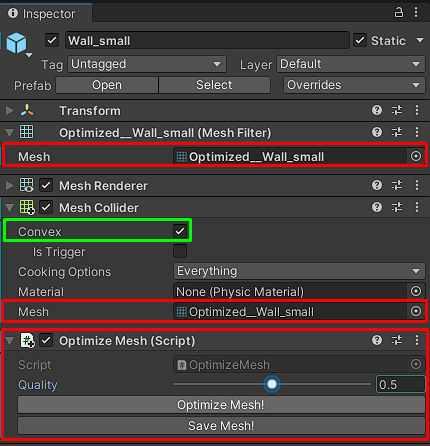
\includegraphics[scale=0.7]{Images/meshOptimization.png}
    \caption{Możliwe sposoby na optymalizację mesha obiektu}
\end{figure}

%\subsubsection{Łączenie Meshów}
% Mesh Combining to technika łączenia wielu meshów w jeden, co może znacząco zredukować liczbę wywołań renderowania. Omówimy, kiedy warto zastosować tę technikę i jak ją zaimplementować.
% To-Do In-Game as well